Neural networks, as outlined in this chapter’s structure, are central to modern machine learning.
Before discussing specific architectures or training procedures, we first provide a structured overview of neural networks as function approximators. 
This includes their basic components—neurons and layers—and the way they are composed into deep architectures.
The goal is to provide an intuitive understanding of how they operate as function approximators by passing data through layers of interconnected units.
This intuition is supported by the \emph{Universal Approximation Theorem}, which states that even a feedforward network with a single hidden layyer can napproximate any continuous function on a compact subset of $\mathbb{R}^n$.
After this conceptual overview, we discuss common activation and loss functions, formalize the training process, and conclude the chapter with an overview of different neural network architectures.

In supervised learning, we are given a dataset $\mathcal{D}$ of $N$ input-output pairs 
\[\mathcal{D}:=\{(x_i,y_i)\}_{i=1}^N \subset \mathbb{R}^{D^{(0)}} \times \mathbb{R}^{D^{(L)}},\]
where each input $x_i\in \mathbb{R}^{D^{(0)}}$ represents a data point with $D^{(0)}$ features, and each $y_i\in \mathbb{R}^{D^{(L)}}$ is the corresponding target or label.
A neural network defines a function \[f:\mathbb{R}^{D^{(0)}} \to \mathbb{R}^{D^{(L)}}\] that aims to approximate the relationship between inputs and outputs.

This function $f$ is represented, as in Cotterell et al.~\cite{cotterell_formal_2024}, as a composition of layer-wise transformations: 
\[
f = f^{(L)} \circ f^{(L-1)} \circ \dots \circ f^{(1)}.
\]
Each function \( f^{(\ell)} : \mathbb{R}^{D^{(\ell-1)}} \rightarrow \mathbb{R}^{D^{(\ell)}} \), for \( \ell = 1, \dots, L \), represents a single layer of the network, where \( D^{(\ell)} \) denotes the number of neurons in layer \( \ell \).  
Each layer consists of a linear transformation followed by a non-linear activation function.
The architecture of the network is defined by the number of layers, their types and their respective with, i.e, the dimension $\mathbb{R}^{D^{(0)}}, ..., \mathbb{R}^{D^{(L)}}$

The final layer \( f^{(L)} \) produces the network’s output, so that the entire network is defined as a composition:
\[
f(x) := f^{(L)} \circ f^{(L-1)} \circ \dots \circ f^{(1)}(x).
\]
The total number of layers \( L \) is called the \emph{depth} of the network.

Given an input \( x_i \in \mathbb{R}^{D^{(0)}} \), the output of the network is the prediction
\[
\hat{y}_i := f(x_i), \quad i = 1, \dots, N.
\]

%The full input space \( \{ x_n \}_{n=1}^N \) is referred to as the feature space, and the set \( \{y_n \}_{n=1}^N \subset \mathbb{R}^{D^{(L)}} \) form the prediction space of the network. 

A neural network is composed of the following types of layers, this is illustrated in Figure ~\ref{fig:IlNN}:
\begin{itemize}
   \item \textbf{Input layer} represents the feature vector \( x \in \mathbb{R}^{D^{(0)}} \) and serves as the entry point of the network. It does not perform any computation itself.
    %\item \textbf{Hidden layers} are the layer where all nontrivial computation occurs. Each hidden layer transforms its input via an affine map followed ba a nonlinear activation function.
    \item \textbf{Hidden layers} are responsible for transforming representations through combinations of parameterized operations and nonlinearities, enabling the network to learn complex functions from data. 
    \item \textbf{Output layer} produces the final prediction $f(x) \in \mathbb{R}^{D^{(L)}}$
\end{itemize}


\begin{figure}[h]
    \centering
    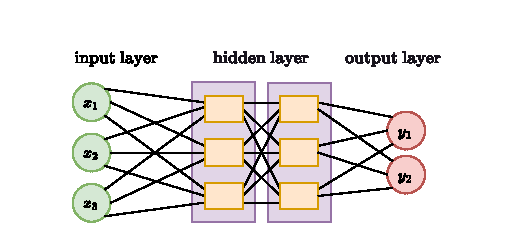
\includegraphics[width=0.7\linewidth]{Abschlussarbeit/Pictures/NN_mathematischausgerichtet.pdf}
    \caption{Illustration of a neural network. Adapted from \cite{zhou_machine_2021}.}
    \label{fig:IlNN}
\end{figure}

To understand the functional building blocks of neural networks, we now examine the internal structure of a single layer.
As illustrated in Figure~\ref{fig:layer}, a layer consists of multiple neurons that receive the same input vector \( x \in \mathbb{R}^{D^{(0)}} \), but apply different parameters.
If the layer comprises \( D^{(L)} \) neurons, that is, it produces an output vector of dimension \( D^{(L)} \), its parameters consist of a weight matrix \( W \in \mathbb{R}^{D^{(L)} \times D^{(0)}} \) and a bias vector \( b \in \mathbb{R}^{D^{(L)}} \).

The output of the layer is a vector \( y \in \mathbb{R}^{D^{(L)}} \), computed as
\[
z := Wx + b, \quad y := \sigma(z),
\]
where \( \sigma \) denotes the activation function, which is applied element-wise.

\begin{figure}[H]
    \centering
    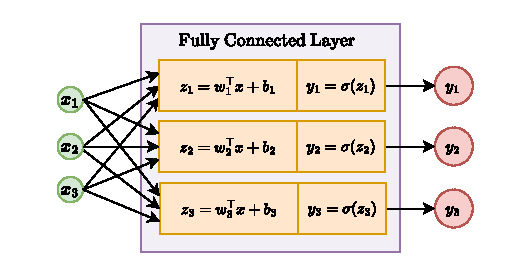
\includegraphics[width=0.7\linewidth]{Abschlussarbeit/Pictures/Layer_outp.pdf}
    \caption{Illustration of a neural networks layer}
    \label{fig:layer}
\end{figure}

At the core of each layer is the artificial neuron.
It performs a simple tow-step operation:
\begin{enumerate}
    \item Compute an affine transormation of the input,
    \item Apply a nonliear activation function.
\end{enumerate}

%Following Stevens et al.~\cite{antiga_deep_2020} notion, a single artificial neuron takes an input vector \( x = (x_1, x_2, \dots, x_n)^\top \in \mathbb{R}^n \), weights \( w = (w_1, w_2, \dots, w_n) \in \mathbb{R}^n \) and a bias term \( b \in \mathbb{R} \), and produces an output:
%\[
%y := \sigma(w^\top x + b).
%\]
%This defines a function \( f \colon \mathbb{R}^n \to \mathbb{R} \), where the codomain \( \operatorname{Im}(f) \) depends on the choice of \( \sigma \).  
%Typical activation functions and their properties are discussed in detail in Section~\ref{ActFunc}.  
%Figure~\ref{fig:artNeuron} shows an artificial neuron.





%\begin{figure}[h]
%    \centering
%    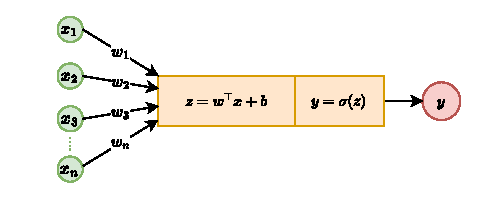
\includegraphics[width=0.7\linewidth]{Abschlussarbeit/Pictures/ArtificialNeuron_output.pdf}
%    \caption{Illustration of a neural networks artificial neuron}
%    \label{fig:artNeuron}
%\end{figure}


